\documentclass[12pt,]{article}
\usepackage{lmodern}
\usepackage{amssymb,amsmath}
\usepackage{ifxetex,ifluatex}
\usepackage{fixltx2e} % provides \textsubscript
\ifnum 0\ifxetex 1\fi\ifluatex 1\fi=0 % if pdftex
  \usepackage[T1]{fontenc}
  \usepackage[utf8]{inputenc}
\else % if luatex or xelatex
  \ifxetex
    \usepackage{mathspec}
  \else
    \usepackage{fontspec}
  \fi
  \defaultfontfeatures{Ligatures=TeX,Scale=MatchLowercase}
\fi
% use upquote if available, for straight quotes in verbatim environments
\IfFileExists{upquote.sty}{\usepackage{upquote}}{}
% use microtype if available
\IfFileExists{microtype.sty}{%
\usepackage{microtype}
\UseMicrotypeSet[protrusion]{basicmath} % disable protrusion for tt fonts
}{}
\usepackage[left=3cm,right=2cm,top=2.5cm,bottom=2cm]{geometry}
\usepackage{hyperref}
\hypersetup{unicode=true,
            pdftitle={Example for using RMarkdown to create scientific manuscripts},
            pdfauthor={Jörn Alexander Quent},
            pdfborder={0 0 0},
            breaklinks=true}
\urlstyle{same}  % don't use monospace font for urls
\usepackage{graphicx,grffile}
\makeatletter
\def\maxwidth{\ifdim\Gin@nat@width>\linewidth\linewidth\else\Gin@nat@width\fi}
\def\maxheight{\ifdim\Gin@nat@height>\textheight\textheight\else\Gin@nat@height\fi}
\makeatother
% Scale images if necessary, so that they will not overflow the page
% margins by default, and it is still possible to overwrite the defaults
% using explicit options in \includegraphics[width, height, ...]{}
\setkeys{Gin}{width=\maxwidth,height=\maxheight,keepaspectratio}
\IfFileExists{parskip.sty}{%
\usepackage{parskip}
}{% else
\setlength{\parindent}{0pt}
\setlength{\parskip}{6pt plus 2pt minus 1pt}
}
\setlength{\emergencystretch}{3em}  % prevent overfull lines
\providecommand{\tightlist}{%
  \setlength{\itemsep}{0pt}\setlength{\parskip}{0pt}}
\setcounter{secnumdepth}{0}
% Redefines (sub)paragraphs to behave more like sections
\ifx\paragraph\undefined\else
\let\oldparagraph\paragraph
\renewcommand{\paragraph}[1]{\oldparagraph{#1}\mbox{}}
\fi
\ifx\subparagraph\undefined\else
\let\oldsubparagraph\subparagraph
\renewcommand{\subparagraph}[1]{\oldsubparagraph{#1}\mbox{}}
\fi

%%% Use protect on footnotes to avoid problems with footnotes in titles
\let\rmarkdownfootnote\footnote%
\def\footnote{\protect\rmarkdownfootnote}

%%% Change title format to be more compact
\usepackage{titling}

% Create subtitle command for use in maketitle
\newcommand{\subtitle}[1]{
  \posttitle{
    \begin{center}\large#1\end{center}
    }
}

\setlength{\droptitle}{-2em}
  \title{Example for using RMarkdown to create scientific manuscripts}
  \pretitle{\vspace{\droptitle}\centering\huge}
  \posttitle{\par}
  \author{Jörn Alexander Quent}
  \preauthor{\centering\large\emph}
  \postauthor{\par}
  \predate{\centering\large\emph}
  \postdate{\par}
  \date{November 29, 2017}

\usepackage{setspace}
\onehalfspacing

\begin{document}
\maketitle
\begin{abstract}
Lorem ipsum dolor sit amet, consectetur adipiscing elit, sed do eiusmod
tempor incididunt ut labore et dolore magna aliqua. Ut enim ad minim
veniam, quis nostrud exercitation ullamco laboris nisi ut aliquip ex ea
commodo consequat. Duis aute irure dolor in reprehenderit in voluptate
velit esse cillum dolore eu fugiat nulla pariatur. Excepteur sint
occaecat cupidatat non proident, sunt in culpa qui officia deserunt
mollit anim id est laborum.
\end{abstract}

{
\setcounter{tocdepth}{3}
\tableofcontents
}
\section{Your fancy formulas}\label{your-fancy-formulas}

You are able to create fancy formulars by innserting LaTex bits
surrounded by \$ signs. Today, we will use a correlation:
\[r = \frac{\Sigma(x_i - \bar{x})(y_i - \bar{y})}{\sqrt{\Sigma(x_i - \bar{x})^2\Sigma(y_i - \bar{y})^2}}\]

\subsection{Analysis}\label{analysis}

Use r chunks for your analysis and use the results later.

\subsection{Report your stats}\label{report-your-stats}

The loaded example data give the speed of cars and the distances taken
to stop. The correlation between these two variables is significant,
\emph{r} = .807, \emph{p} \textless{} .001.

\subsubsection{Show your graphs}\label{show-your-graphs}

You add nicely rendered graphs to your text. For that it is important to
specify that you want the respected chunk to be included but not echoed.

\begin{figure}[htbp]
\centering
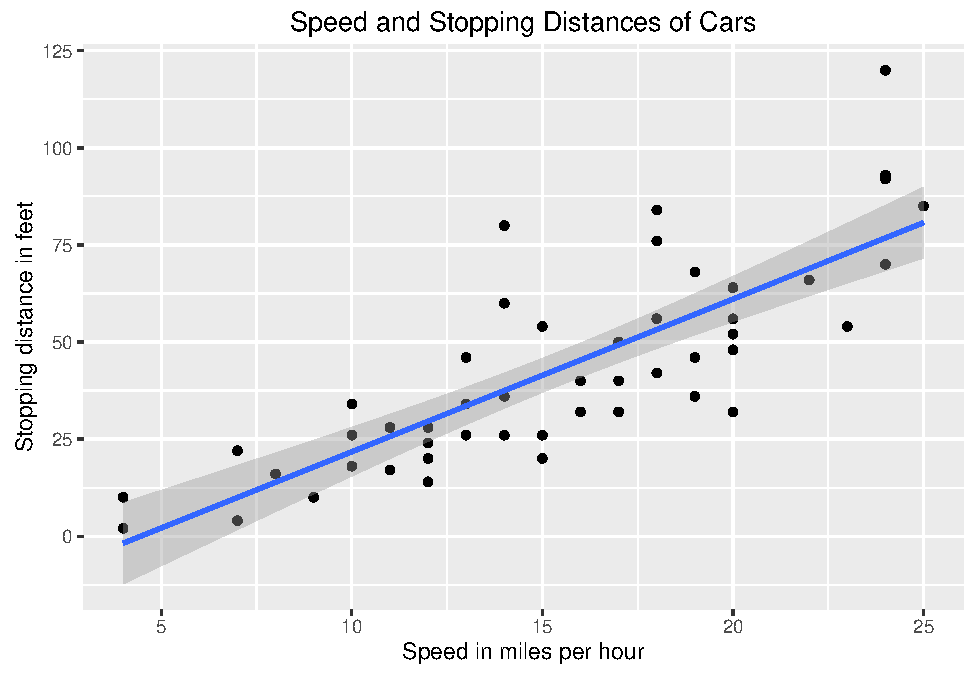
\includegraphics{methodsDay2017_example_files/figure-latex/unnamed-chunk-2-1.pdf}
\caption{There is a significant correlation between the speed of a car
and the distance it needs to stop, \emph{r} = .807 , \emph{p}
\textless{} .001 .}
\end{figure}

\section{Writing your text and cite}\label{writing-your-text-and-cite}

The nice thing about RMarkdown is that you can write the whole
manuscript with that includes using citations. You can have the standard
way of citing at the end of a sentence (Quent, 2017a, 2017b). As Quent
(2017a) shows, you can also have it that way. Most reference management
software (e.g.~Zotero or Mendeley) alow you to export the refereneces in
BibTeX format. In this case, the references are saved in BibTeX format
in the references.bib file.

\section*{References}\label{references}
\addcontentsline{toc}{section}{References}

\hypertarget{refs}{}
\hypertarget{ref-Quent2017a}{}
Quent, J. A. (2017a). This is a title. \emph{Made up journal},
\emph{1}(1), 1--2.

\hypertarget{ref-Quent2017b}{}
Quent, J. A. (2017b). This is another title. \emph{Proceedings in the
world of fantasy}, \emph{3}(10), 44--99.


\end{document}
